\documentclass[12pt]{article}
\usepackage[margin=1in,letterpaper]{geometry}
\usepackage[utf8]{inputenc}
\usepackage[T1]{fontenc}
\usepackage{graphicx}
\usepackage{amssymb}
\usepackage{amsmath}
\usepackage{palatino}
\usepackage{mathpazo}
\usepackage{color}
\usepackage{hyperref}
\usepackage{multirow}
\usepackage{braket}
\usepackage{relsize}
\usepackage{color, colortbl}
\usepackage{booktabs}
\usepackage[dvipsnames]{xcolor}
\definecolor{darkblue}{RGB}{46,48,147}
\hypersetup{colorlinks=true,
            linkcolor=darkblue,
            urlcolor=darkblue,
            citecolor=darkblue}
\definecolor{Gray}{gray}{0.9}
\definecolor{LightCyan}{rgb}{0.88,1,1}
\definecolor{LightRed}{rgb}{1,0.92,0.92}
\newcommand{\solColor}{blue}
\newcommand{\sol}{\color{\solColor}}
\newcommand*\publistbasestyle{phys}
\usepackage[style=publist,
biblabel=brackets,
sorting=dt,
plauthorhandling=highlight,
nameorder=given-family,
]{biblatex}
\DeclareSourcemap{
 \maps[datatype=bibtex,overwrite=true]{
  \map{
    \step[fieldsource=Collaboration, final=true]
    \step[fieldset=usera, origfieldval, final=true]
  }
 }
}
\renewbibmacro*{author}{
  \iffieldundef{usera}{
    \printnames{author}
  }{
    \printfield{usera} Collaboration
  }
}
\addbibresource{syllabus.bib}

\begin{document}

\begin{center}
	\textbf{University of California San Diego\\
		Department of Physics\\
		Physics 139/239, Spring 2024\\
		Machine Learning in Physics (4 units)}
\end{center}

\begin{figure}[h!]
	\centering
	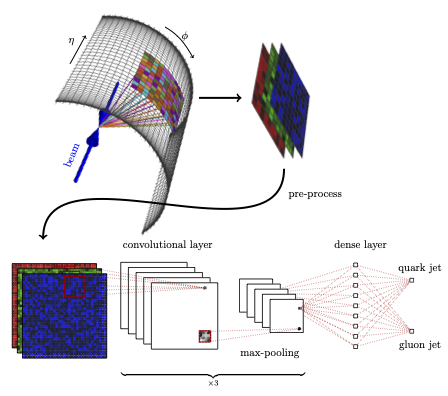
\includegraphics[width=0.7\textwidth]{quark_gluon.pdf}
\end{figure}

\noindent\textbf{Instructors}:\\
Javier Duarte, \href{mailto:jduarte@ucsd.edu}{jduarte@ucsd.edu}, OH M 11:00a--12:00p, MYR-A 5513\\
Aobo Li, \href{mailto:aol002@ucsd.edu}{aol002@ucsd.edu}, OH W 1:00--2:00p, MYR-A 4571\\
\noindent \textbf{Teaching assistant}: Anthony Aportela, \href{mailto:aaportel@ucsd.edu}{aaportel@ucsd.edu}, OH F 11:00a--12:00p, MYR-A 5516\\

\noindent\textbf{Course webpage, Zoom link to lectures}:\\
\hspace*{1cm}Canvas: \href{https://canvas.ucsd.edu/courses/56257}{https://canvas.ucsd.edu/courses/56257}\\
\hspace*{1cm}Webpage: \href{https://jduarte.physics.ucsd.edu/phys139\_239}{https://jduarte.physics.ucsd.edu/phys139\_239}\\
\hspace*{1cm}All assignments will be due through Canvas and Gradescope (accessed through Canvas).\\

\begin{center}
	\rule{\textwidth}{0.5pt}
\end{center}

\noindent\textbf{Course information}: This course is an upper-division undergraduate course and introductory graduate course on machine learning in physics.
No previous machine learning knowledge is necessary.
However, some basic knowledge of calculus, linear algebra, statistics, and Python programming may be expected/useful.

The course structure will consist of weekly lectures on conceptual topics, e.g. statistics, linear algebra, scientific data set exploration, feature engineering, (stochastic) gradient descent, neural networks, and unsupervised learning.
Students will learn key concepts in data science and machine learning, including selecting and preprocessing data, designing machine learning models, evaluating model performance, and relating model inputs and outputs to the underlying physics concepts.
We will apply these methods to the domains of collider physics, neutrino physics, astronomy, and potentially others.
There will be 4 homework assignments.
There will also be a final project in which students will work in groups to reproduce the results of an ML in physics research article.
A midterm assignment to propose the project will also be required.

\begin{center}
	\rule{\textwidth}{0.5pt}
\end{center}

\noindent\textbf{Schedule}:
\begin{center}
	\begin{tabular}{|l|c|l|m{60mm}|}
		\hline
		Lecture    & MWF         & 10--10:50a   & PCYNH	121, Zoom \href{https://ucsd.zoom.us/j/96613284864}{96613284864} \\\hline
		Final exam & M 6/10/2024 & 8:00a-10:59p & Location TBD, Zoom TBD                                                 \\\hline
	\end{tabular}
\end{center}

\noindent\textbf{First lecture}: M 4/1/2024

\begin{center}
	\rule{\textwidth}{0.5pt}
\end{center}

\noindent\textbf{Textbook}: There is no required textbook for this course.
At the end of the syllabus, we list a bibliography of (mostly free) textbooks and online resources we will draw from.

\begin{center}
	\rule{\textwidth}{0.5pt}
\end{center}

\noindent\textbf{Student learning outcomes}: Upon successful completion of Physics 139/239, students will be able to:
\begin{itemize}
	\item Find, explore, select, and preprocess scientific data
	\item Choose and design machine learning models
	\item Evaluate model performance and compare to standard benchmarks
	\item Debug machine learning workflows
	\item Relate model inputs and outputs to underlying physics concepts
	\item Collaborate with peers to tackle complex, realistic problems
	\item Present findings
\end{itemize}

\begin{center}
	\rule{\textwidth}{0.5pt}
\end{center}

\noindent\textbf{Grading policy}: Your final course grade will be determined according to the following:
\begin{itemize}
	\item 50\% Homework.
	\item 10\% Participation in class, via Slack, and completion of exit tickets.
	\item 20\% Midterm: Written proposal for group project.
	\item 20\% Final: Written group project summary, presentation, self/peer evaluations, and code.
\end{itemize}

\begin{center}
	\rule{\textwidth}{0.5pt}
\end{center}

\noindent\textbf{Drop policy}: The lowest homework score is dropped automatically.
This drop policy is designed to account for any illnesses, family, medical, mental, or other emergencies.

If you have an extended emergency (e.g., a long hospital stay) that hinders your ability to turn complete assignments beyond the emergency policy allowance, contact the professor directly as soon as the situation arises.

\begin{center}
	\rule{\textwidth}{0.5pt}
\end{center}

\noindent\textbf{Discussion board}: We will use Slack: \href{https://join.slack.com/t/ucsdphys139/shared\_invite/zt-110gwd4lx-pZBsItfcxhbOD5BV6afVDA}{ucsdphys139.slack.com}

\begin{center}
	\rule{\textwidth}{0.5pt}
\end{center}

\noindent\textbf{Homework}: Each homework will consist of a set of conceptual and programming problems.
The assignments will be submitted as Jupyter notebooks or GitHub repositories.

There will be a first deadline (on Fridays at 8:00pm) to submit the homework, which will be graded based on effort and completeness.

There will be a second deadline (on Wednesdays at 8:00pm) to submit corrections for the homework, which will be graded based on effort and correctness.

\begin{center}
	\rule{\textwidth}{0.5pt}
\end{center}

\noindent\textbf{Midterm and final project}:
For the final project, students will work in groups of $\sim$4 to reproduce or extend the results of an ML in physics research article.
Some candidate articles are listed at the end of the syllabus.
The final project deliverables are: (1) a 4-page paper on the project, (2) code provided as a public GitHub repository, (3) a 10-minute presentation by all members of the group during finals week, and (4) self and peer evaluations for group contributions.
Students will also be required to submit a 1-page written proposal for the project in Week 7.
This is to ensure the project is feasible and to receive feedback from the instructors.

\begin{center}
	\rule{\textwidth}{0.5pt}
\end{center}

\noindent\textbf{Attendance (lectures)}: In-person lecture attendance is not required, but strongly recommended.
The lecture hours will be split into conceptual and hands-on portions, with interactive problem-solving and pair programming throughout.
Please, bring a laptop that you can program with to lecture.
If you do not have one, please contact the instructor, and we will help you.
These sessions will be recorded.

\emph{Exit tickets}: At the end of each class, you will be invited to fill out an \href{https://forms.gle/4DmG5SjBUEM5pe6U8}{exit ticket}.

\begin{center}
	\rule{\textwidth}{0.5pt}
\end{center}

\noindent\textbf{Academic integrity}: Please read the College Policies section of the \href{http://senate.ucsd.edu/Operating-Procedures/Senate-Manual/Appendices/2}{UCSD's Policy on Integrity of Scholarship}.
These rules will be enforced.
Cheating includes, but is not limited to: submitting another person's work as your own, copying from any person/source, and using any unauthorized materials or aids during exams.

For homework assignments, copying from an online solution, a peer's solution, a Chegg solution, or shared work (on Discord, for example) is considered cheating.
Collaboration is encouraged, but by the time you start writing your own solution to turn in, you should not be looking at any other source.
You should know the rough outline of the solution well enough that you do not need to reference something line-by-line.
Plagiarizing a solution but changing variable names is considered cheating.
Soliciting help online via Chegg, Quora, etc. is considered cheating.
If suspected, you might be asked to rework similar problems in a Zoom one-on-one meeting with the instructor and/or TA.

Any questions on what constitutes an academic integrity violation should be addressed to the instructor; any violation of academic integrity will result in immediate reporting to the UCSD Office of Academic Integrity, and can result in an automatic ``F'' for the course at the discretion of the instructor.

\begin{center}
	\rule{\textwidth}{0.5pt}
\end{center}

\noindent\textbf{Counseling and Psychological Services (CAPS):} The mission of CAPS is to promote the personal, social, and emotional growth of students.
Many services are available to UCSD students including individual, couples, and family counseling, groups, workshops, and forums, consultations and outreach, psychiatry, and peer education.
To make an appointment, call (858) 534-755.
For more information, visit \href{https://wellness.ucsd.edu/caps/}{https://wellness.ucsd.edu/caps/}.

\begin{center}
	\rule{\textwidth}{0.5pt}
\end{center}

\noindent\textbf{\emph{Schedule}} (Subject to change):\\

\noindent\textbf{Week 1}

\emph{Monday 4/1 (Li)}: \underline{Lecture 01}: Course overview, introduction to ML, linear regression; Homework 1 released

\emph{Wednesday 4/3 (Li)}: \underline{Lecture 02}: Over/underfitting, bias-variance tradeoff, cross validation

\emph{Friday 4/5 (Li)}: \underline{Lecture 03}: Perceptron learning algorithm, (stochastic) gradient descent; \underline{Hands-on}: Python/Jupyter, NumPy, Git, debugging

\noindent\textbf{Week 2}

\emph{Monday 4/8 (Duarte)}: \underline{Lecture 04}: Support vector machine

\emph{Wednesday 4/10 (Duarte)}: \underline{Lecture 05}: Regularization, logistic regression

\emph{Friday 4/12 (Duarte)}: Homework 1 due; \underline{Lecture 06}: (Boosted) decision trees

\noindent\textbf{Week 3}

\emph{Monday 4/15 (Li/Duarte)}: \underline{Lecture 07}: (Boosted) decision trees (cont.); \underline{Hands-on}: Scikit-learn, XGBoost, classifying Higgs boson events

\emph{Wednesday 4/17 (Li)}: Homework 1 (corrections) due; Homework 2 released; \underline{Lecture 08}: (Deep) neural networks, backpropagation

\emph{Friday 4/19 (Li)}: \underline{Lecture 09}: Classification metrics, confusion matrix, ROC curve, AUC

\noindent\textbf{Week 4}

\emph{Monday 4/22 (Duarte)}: \underline{Lecture 10}: (Deep) neural networks (cont.), training issue, data standardization; \underline{Hands-on}: Keras, classifying jets with high-level features

\emph{Wednesday 4/24 (Duarte)}: \underline{Lecture 11}: Optimizers: (Nesterov) momentum, RMSProp, Adam, skip connections, regularization: dropout, early stopping

\emph{Friday 4/26 (Li)}: Homework 2 due; \underline{Lecture 12}: Types of data, inductive bias, image-like data, convolutional neural networks

\noindent\textbf{Week 5}

\emph{Monday 4/29 (Li)}: \underline{Lecture 13}: Convolutional neural networks (cont.)

\emph{Wednesday 5/1 (Li)}: Homework 2 (corrections) due; Homework 3 released; \underline{Lecture 14}: Spherical convolutional neural networks

\emph{Friday 5/3 (Duarte)}: \underline{Hands-on}: Keras, classifying astronomical data (images)

\noindent\textbf{Week 6}

\emph{Monday 5/6 (Li)}: \underline{Lecture 15}: Time-series data, recurrent neural networks

\emph{Wednesday 5/8 (Li)}: \underline{Lecture 16}: Recurrent neural networks (cont.)

\emph{Friday 5/10 (Li)}: Homework 3 due; \underline{Hands-on}: Identifying radio signals (time series)

\noindent\textbf{Week 7}

\emph{Monday 5/13 (Duarte)}: \underline{Lecture 18}: Point cloud and graph-like data, relational inductive bias, permutation invariance/equivariance, graph neural networks

\emph{Wednesday 5/15 (Duarte)}: Homework 3 (corrections) due; \underline{Lecture 19}: Graph neural networks (cont.)

\emph{Friday 5/17 (Duarte)}: Project proposal due; \underline{Hands-on}: Spektral, $N$-body simulations, springs

\noindent\textbf{Week 8}

\emph{Monday 5/20 (Li)}: \underline{Lecture 21}: Unsupervised learning, clustering

\emph{Wednesday 5/22 (Li)}: \underline{Lecture 22}: Autoencoders, variational autoencoders

\emph{Friday 5/24 (Li)}: Homework 4 due; \underline{Lecture 23}: \underline{Hands-on}: Finding anomalies in LHC/LIGO data

\noindent\textbf{Week 9}

\emph{Wednesday 5/29 (Duarte)}: Homework 4 (corrections) due; \underline{Lecture 24}: Model compression, pruning

\emph{Friday 5/31 (Duarte)}: \underline{Lecture 25}: Quantization

\noindent\textbf{Week 10}

\emph{Monday 6/3 (Duarte)}: Knowledge distillation

\emph{Wednesday 6/5 (Duarte)}: \underline{Hands-on}: TensorFlow Model Optimization, QKeras

\emph{Wednesday 6/7 (Guest)}: \underline{Guest lecture}: TBD

\noindent\textbf{Finals Week}

\emph{Monday 6/10}: Final project due

\begin{center}
	\rule{\textwidth}{0.5pt}
\end{center}

\noindent\textbf{\emph{Bibliography}}:\\

\textbf{Textbooks:}

\newrefsection
\nocite{Mehta:2019,Abu-Mostafa:2012,Erdman:2021,Zeljko:2014,Calafiura:2022,Chollet:2021,Goodfellow-et-al-2016}
\printbibliography[heading=none]

\textbf{Videos:}

\newrefsection
\nocite{3blue1brown_neuralnetwork,3blue1brown_gradientdescent}
\printbibliography[heading=none]

\textbf{Reviews:}

\newrefsection
\nocite{Carleo:2019ptp,hepmllivingreview}
\printbibliography[heading=none]

\textbf{Candidate articles for final project:}

\newrefsection
\nocite{deOliveira:2015xxd,Aurisano:2016jvx,Komiske:2016rsd,Khan:2018opv,Zhou:2019,Moreno:2019neq,Ormiston:2020ele,Moreno:2021fvp,Erdmann:2019nie,Guest:2016iqz,Majorana:2023kmv}
\printbibliography[heading=none]

\textbf{Public datasets:}

\newrefsection
\nocite{kasieczka_gregor_2019_2603256,hbb_dataset,galaxy-zoo-the-galaxy-challenge,g2net-gravitational-wave-detection,trackml-particle-identification,majorana_collaboration_2023_8257027}
\printbibliography[heading=none]

\end{document}
